\title{EE5311 -- Assignment 7}
\author{Joyen Benitto}
\date{\today}
\maketitle

\section{Problem 1(a): schematic delays}

\subsubsection{Schematic}

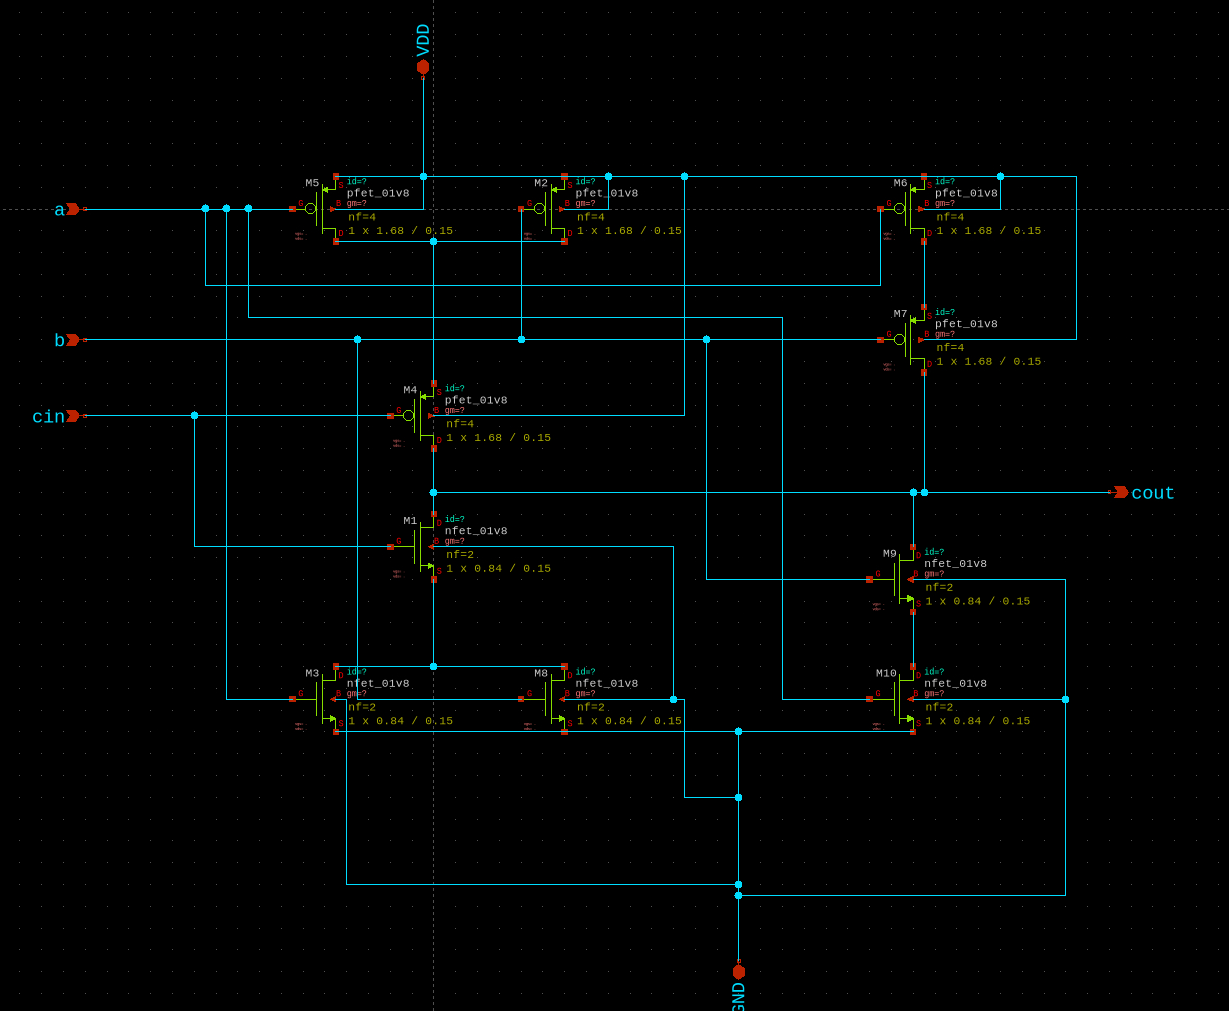
\includegraphics[width=0.9\textwidth]{figures/carry_schematic.png}

\textbf{Figure 1:} \texttt{carry.sch} -- mirror carry, nMOS $0.84/0.15$, pMOS $1.68/0.15$

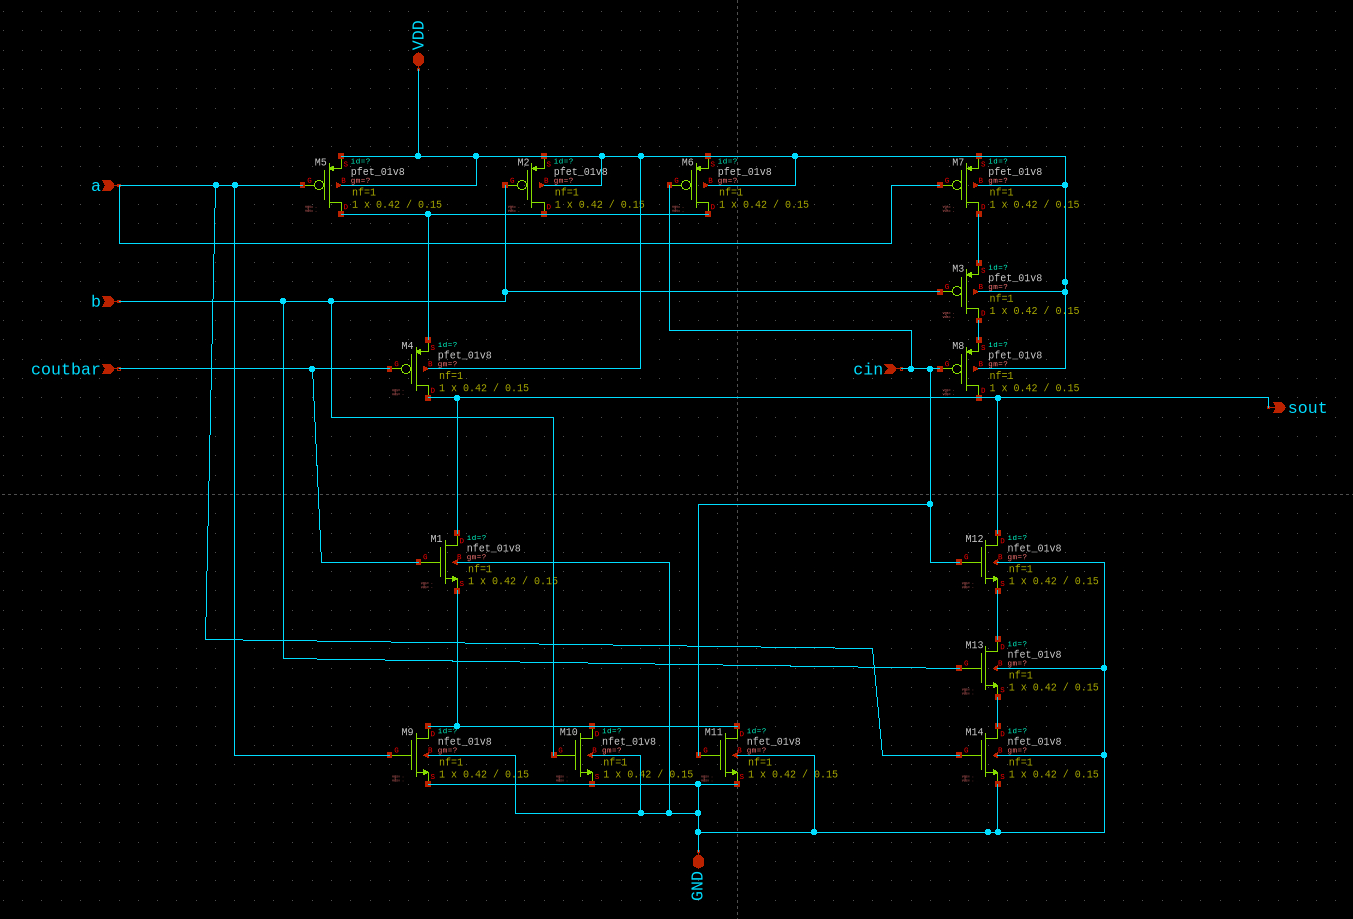
\includegraphics[width=0.9\textwidth]{figures/sum_schematic.png}

\textbf{Figure 2:} \texttt{sum.sch} -- mirror sum, all devices $0.42/0.15$

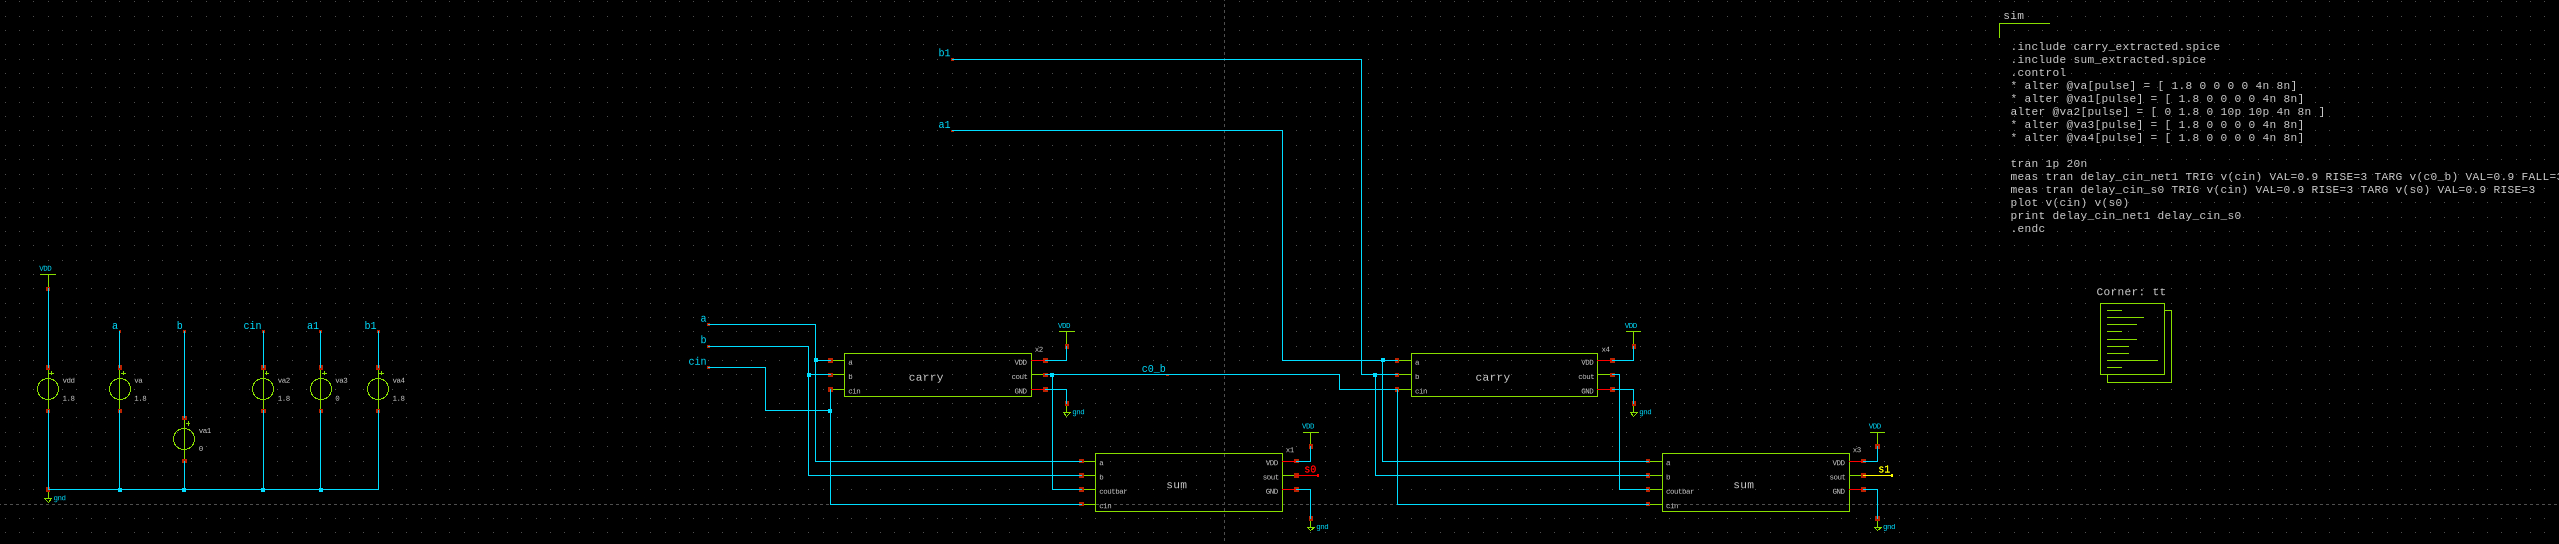
\includegraphics[width=0.95\textwidth]{figures/tb_schematic.png}

\textbf{Figure 3:} two-stage ripple testbench (\texttt{assign1a.sch}, schematic and extracted netlists)

\subsubsection{Sizing}

Widths in units of the minimum width $0.42\ \mu\text{m}$; the reference inverter has $W_p=2$, $W_n=1$.
\[
g = \frac{C_{in,carry}}{C_{inv}} = \frac{4+2}{3} = 2, \qquad
b = \frac{C_{on-path}+C_{off-path}}{C_{on-path}} = \frac{6+6}{6} = 2
\]
\[
f = g\,b\,h = 4 \;\Rightarrow\; 4 = 2\cdot2\cdot h \;\Rightarrow\; h = 1 \;\Rightarrow\; \alpha = 1
\]
\[
W_p = 4\alpha\cdot0.42 = 1.68\ \mu\text{m}\ (n_f=4), \qquad
W_n = 2\alpha\cdot0.42 = 0.84\ \mu\text{m}\ (n_f=2)
\]

\subsubsection{Measurement}

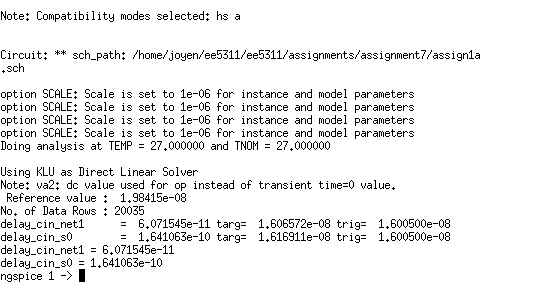
\includegraphics[width=0.85\textwidth]{figures/delay_schematic.png}

\textbf{Figure 4:} ngspice \texttt{.meas} output, schematic netlists

\subsubsection{Calculation}

\[
\begin{aligned}
t_{C_{-1}\to C_0} &= 1.606572\times10^{-8} - 1.600500\times10^{-8} = 60.72\ \text{ps} \\
t_{C_{-1}\to S_0} &= 1.616911\times10^{-8} - 1.600500\times10^{-8} = 164.11\ \text{ps}
\end{aligned}
\]

%%------------------------------------------------------------------------------
\section{Problem 1(b): logical effort}

\subsubsection{Calculation}

Reference inverter ($0.42/0.84$, Assignment 3): two-inverter delay $=36.87$~ps, so
$t_p = 36.87/2 = 18.44$~ps and $t_p = 2\tau \Rightarrow \tau = 9.22$~ps.

Carry ($C_{in}$ input, equal-drive reference inverter $C=1.26\ \mu$m):
\[
g = \frac{0.84+1.68}{1.26} = 2, \qquad p = \frac{5.04}{1.26} = 4
\]
\[
b = \frac{2.52 + (0.84+1.68)}{2.52} = 2, \qquad h = \frac{2.52}{2.52} = 1, \qquad f = gbh = 4
\]
\[
t_{C_{-1}\to C_0} = \tau(gbh+p) = 9.22\,(4+4) = 73.7\ \text{ps}
\]
Sum ($\overline{C_{out}}$ input, two-high stacks, no external load):
\[
g = 2, \quad h = 0, \quad p = 4 \Rightarrow t_{sum} = 4\tau = 36.9\ \text{ps}, \qquad
t_{C_{-1}\to S_0} = 8\tau + 4\tau = 110.6\ \text{ps}
\]

\begin{center}
\begin{tabular}{lcc}
\hline
 & Measured & Logical effort \\
\hline
$C_{-1}\to C_0$ & 60.72~ps & 73.7~ps \\
$C_{-1}\to S_0$ & 164.11~ps & 110.6~ps \\
\hline
\end{tabular}
\end{center}

%%------------------------------------------------------------------------------
\section{Problem 1(c): layout extracted delays}

\subsubsection{Layout}

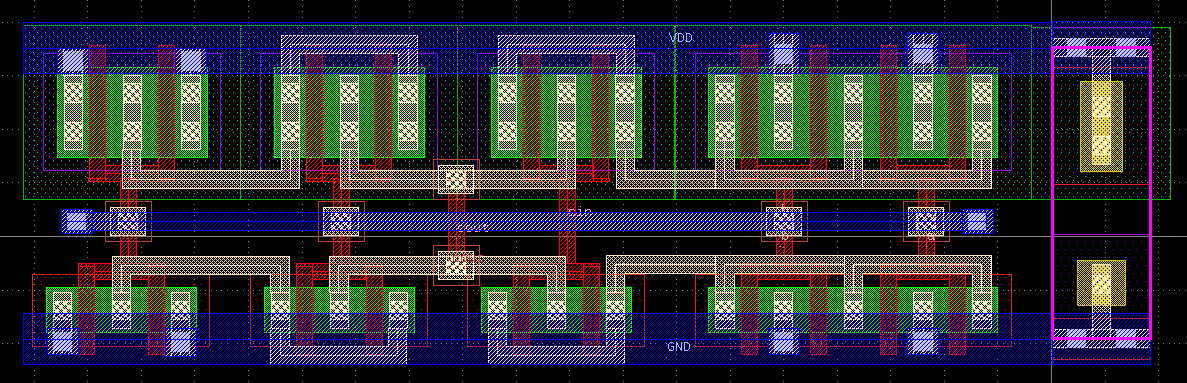
\includegraphics[width=0.7\textwidth]{figures/carry_layout.png}

\textbf{Figure 5:} \texttt{carry.gds}

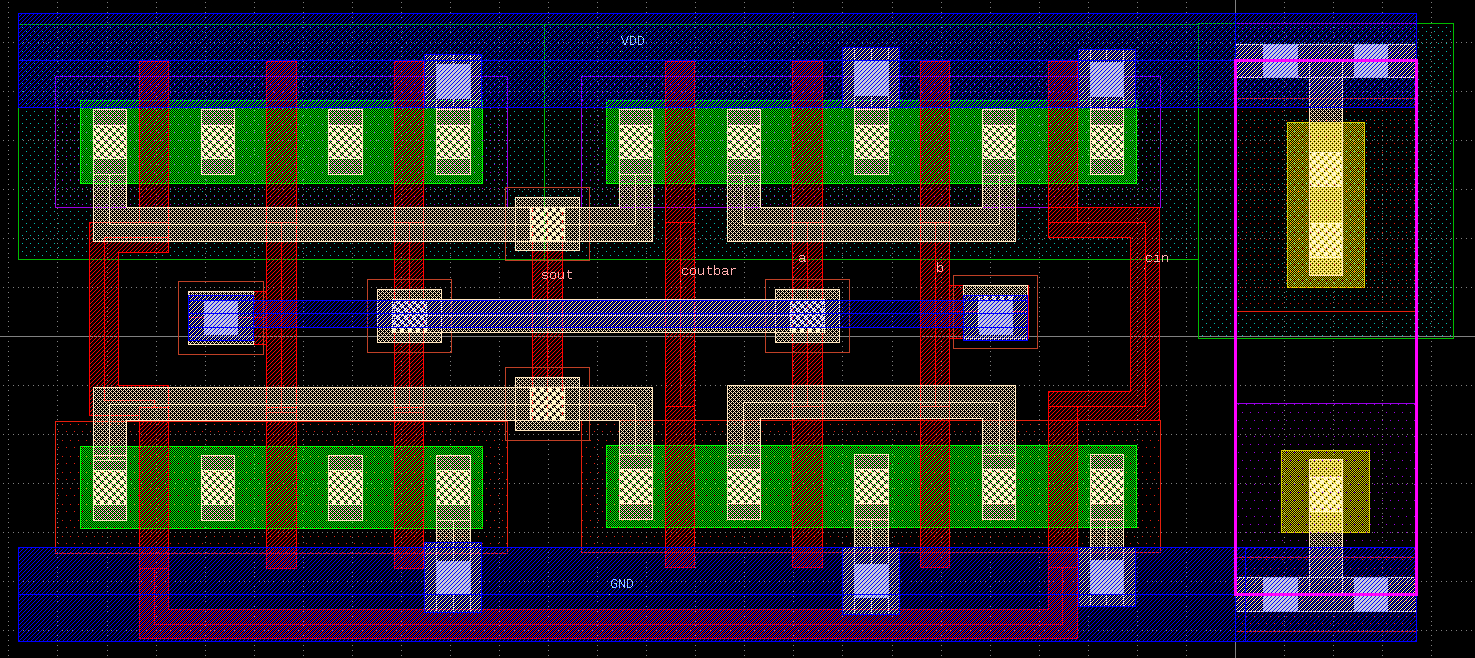
\includegraphics[width=0.7\textwidth]{figures/sum_layout.png}

\textbf{Figure 6:} \texttt{sum.gds}

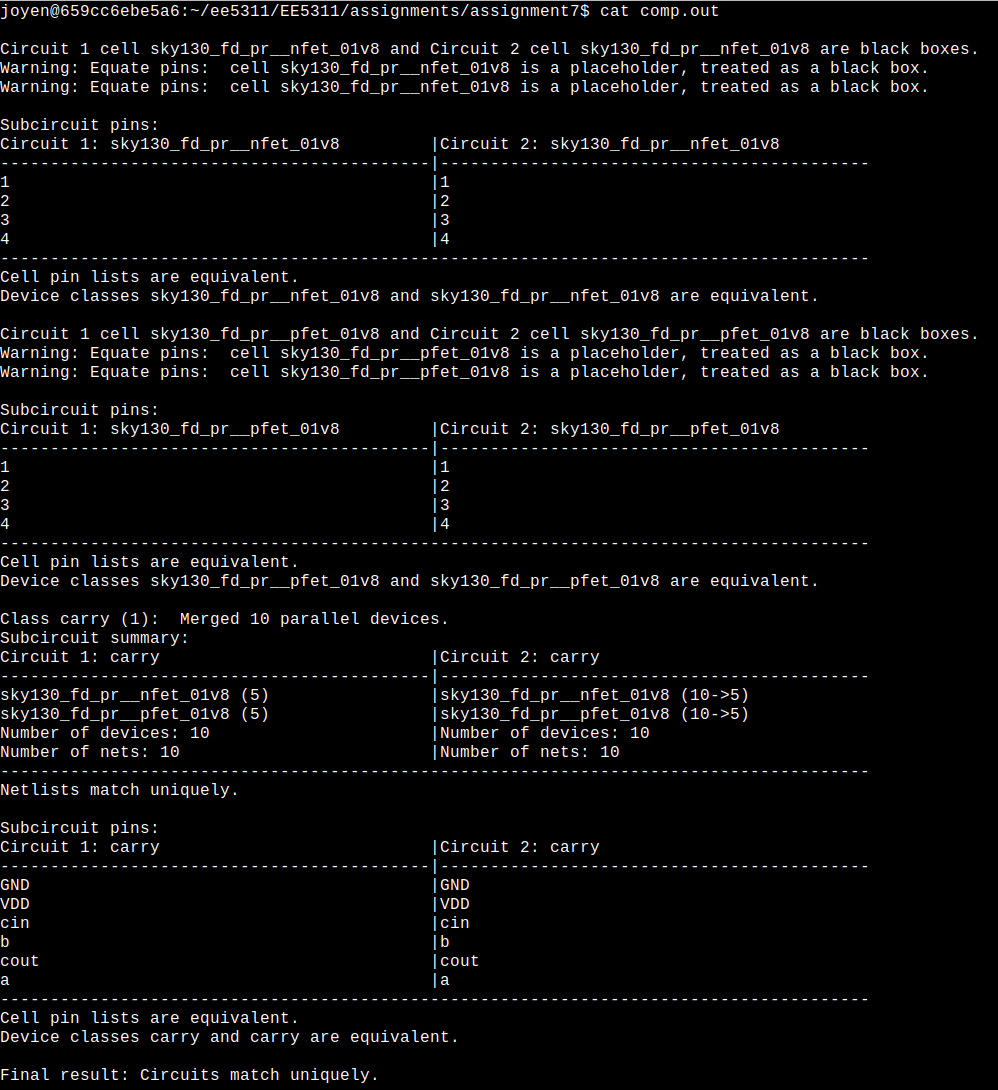
\includegraphics[width=0.7\textwidth]{figures/carry_lvs.png}

\textbf{Figure 7:} \texttt{carry.gds} LVS (\texttt{comp.out}): circuits match uniquely

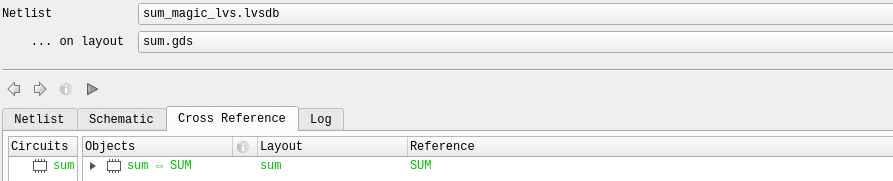
\includegraphics[width=0.7\textwidth]{figures/sum_lvs.png}

\textbf{Figure 8:} \texttt{sum.gds} LVS (KLayout)

\subsubsection{Measurement}

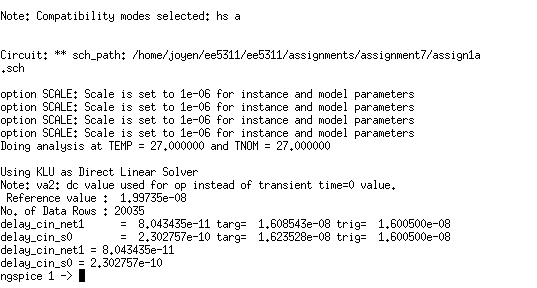
\includegraphics[width=0.85\textwidth]{figures/delay_extracted.png}

\textbf{Figure 9:} ngspice \texttt{.meas} output, layout extracted

\subsubsection{Calculation}

\[
\begin{aligned}
t_{C_{-1}\to C_0} &= 1.608543\times10^{-8} - 1.600500\times10^{-8} = 80.43\ \text{ps} \\
t_{C_{-1}\to S_0} &= 1.623528\times10^{-8} - 1.600500\times10^{-8} = 230.28\ \text{ps}
\end{aligned}
\]

\begin{center}
\begin{tabular}{lccc}
\hline
 & Schematic & Extracted & Increase \\
\hline
$C_{-1}\to C_0$ & 60.72~ps & 80.43~ps & 32.5\% \\
$C_{-1}\to S_0$ & 164.11~ps & 230.28~ps & 40.3\% \\
\hline
\end{tabular}
\end{center}
